\section{Transformada de Fourier}

\subsection{O que é a Transformada de Fourier?}

A transformada de Fourier é uma transformação matemática que "quebra" uma forma de onda (função ou sinal) em uma soma de funções periódicas. A análise de Fourier converte um sinal do seu domínio original para uma representação no domínio da frequência.

Jean-Baptiste Joseph Fourier (Auxerre, 21 de março de 1768 — Paris, 16 de maio de 1830) foi o matemático e físico francês que descobriu que todo sinal pode ser descrito como uma superposição de senóides complexas.

\subsection{Sinais}
Os sinais traduzem a evolução de uma grandeza ao longo do tempo ou espaço e podem ser classificados segundo os critérios:

\begin{itemize}
\item Continuidade: sinais contínuos ou discretos
\item Periodicidade: sinais periódicos ou aperiódicos 
\end{itemize}

\subsubsection{Sinais contínuos}

Um sinal diz-se contínuo se o seu domínio for IR ou um intervalo contínuo de IR. Assim:

\[ x: IR \rightarrow IR \]

\[ x: [a,b] \rightarrow IR \]

- Sinais contínuos são sinais que não possuem espaços distinguíveis entre os seus valores.
- Advém de grandezas que podem ser medidas.

\subsubsection{Sinais discretos}
\begin{itemize}
\item Sinais discretos são sinais que possuem espaços entre os seus valores.
\item Advém de grandezas que são contadas.
\item Só os sinais discretos podem ser armazenados e processados em computadores digitais.
\item Pode-se converter um sinal contínuo num sinal discreto através da coleção de amostras do sinal contínuo.
\end{itemize}

\subsubsection{Sinais periódicos}
Um sinal discreto x(n) é periódico com período $N \ \in \ IN$ se:

\[ \large x(n + N) = x(n), \forall \ n \ \in Z \]

\subsection {Tipos de Abordagens}

De acordo com o tipo de sinal que estamos lidando, existem 4 diferentes tipos de abordagem:
\begin{itemize}
\item Sinais contínuos e aperiódicos: Transformada de Fourier
\item Sinais contínuos e periódicos: Série de Fourier
\item Sinais discretos e aperiódicos: Transformada de Fourier de Tempo Discreto (TFTD)
\item Sinais discretos e periódicos: Transformada Discreta de Fourier (TDF)
\end{itemize}

\subsection {Fórmula para Transformada Discreta de Fourier (DFT)}
Para um sequência finita de valores complexos ou reais $x_{n}$ obtidos pela amostragem de N valores de um sinal contínuo nos instantes $f(0), f(1), f(2), ... f(k), ... f(N-1)$, a Fórmula para a \textbf{Transformada Discreta de Fourier} é: 

\[ \large X_{k} = \sum_{n = 0}^{N-1} x_{n} \cdot e^{-j2\pi\frac{kn}{N}} \]

Sendo $x_{n}$ a amplitude (real ou complexo) de um sinal periódico em um instante de tempo $t$. Tais valores são obtidos por amostragem de uma função periódica contínua. O resultado da fórmula é uma série de números complexos no domínio da frequência.

O TDF se tornou bastante utilizado em computação numérica devido ao algoritmo chamado \textbf{Transformada Rápida de Fourier}, que é um método bastante eficiente para se calcular a Transformada Discreta de Fourier (DFT) e a sua inversa. 

Vamos calcular a Transformada Discreta de Fourier pelo algoritmo rápido usando a função \textbf{fft} da biblioteca Scipy do Python.

\subsection {Transformada Discreta de Fourier (DFT) no Python}
Supondo 2 ondas senoidais de frequências 2Hz e 3Hz. Se somarmos ambas as ondas obteríamos uma onda de forma um pouco mais complicada. Vamos gerar essas 2 ondas e somá-las utilizando o código abaixo:

\begin{minted}{python}
import numpy as np
from matplotlib import pyplot as plt
SAMPLE_RATE = 50 # Hertz
tempo = 10  # Segundos
tempoTicks = [x for x in range(tempo+1)]
f, (ax1, ax2, ax3) = plt.subplots(3, 1, 
sharex=False, figsize=(15,8))
# ajustando a distância vertical entre os plots
f.subplots_adjust(hspace=0.3)
def ondaSeno(freq, sample_rate, tempo, amp = 1):
	# gera 'sample_rate * tempo' amostras
	x = np.linspace(0, tempo, sample_rate * tempo, 
	endpoint=False)
	# multiplica cada amostra pela frequência
	frequencias = x * freq
	# np.sin(ângulo em radianos)
	y = amp*np.sin((2 * np.pi) * frequencias)
	return x, y
ax1.set_title("Função seno (2Hz)")
ax2.set_title("Função seno (3Hz)")
ax3.set_title("Soma das funções senoidais 2Hz e 3Hz")
# Gerando uma onda senoidal de 2Hz
x, y = ondaSeno(2, SAMPLE_RATE, tempo, amp = 3)
# Gerando uma onda senoidal de 3Hz
x1, y1 = ondaSeno(3, SAMPLE_RATE, tempo)
ax1.grid(True, axis = 'x', alpha = 0.7 , 
color = 'black', which='both')
ax2.grid(True, axis = 'x', alpha = 0.7 , 
color = 'black', which='both')
ax3.grid(True, axis = 'x', alpha = 0.7 , 
color = 'black', which='both')
\end{minted}

Continuação...

\begin{minted}{python}
plt.xticks([0,1,2,3,4,5,6,7,8,9,10])
ax1.set_xticks(tempoTicks)
ax2.set_xticks(tempoTicks)
ax3.set_xticks(tempoTicks)
ax1.axhline(y=0, color='black')
ax2.axhline(y=0, color='black')
ax3.axhline(y=0, color='black')
ysoma = y + y1
ax1.plot(x, y, 'tab:red')
ax2.plot(x1, y1, 'tab:blue')
ax3.plot(x1, ysoma, 'tab:orange')
plt.show()
\end{minted}

\begin{figure}[H]
	\centering
	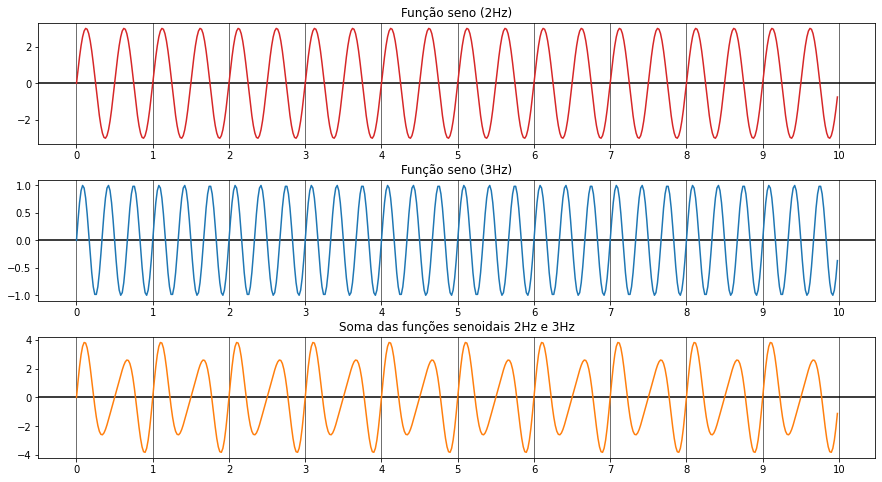
\includegraphics[width=1\textwidth]{./Imagens/Transformada de Fourier/TF1.png} 
	\caption{Soma de senoides}
	\label{fig:TF1}
\end{figure}

A função \textbf{fft} aplicado no sinal resultante retornará uma série de números complexos. Utilizaremos os valores absolutos desses números complexos na plotagem do gráfico. Ainda, esse plot exibirá picos de frequência que nos indicará as frequências dos componentes originais que deu origem ao sinal resultante. 

No exemplo abaixo, os picos de frequências estão em $2Hz$ e $3Hz$.

\begin{figure}[H]
	\centering
	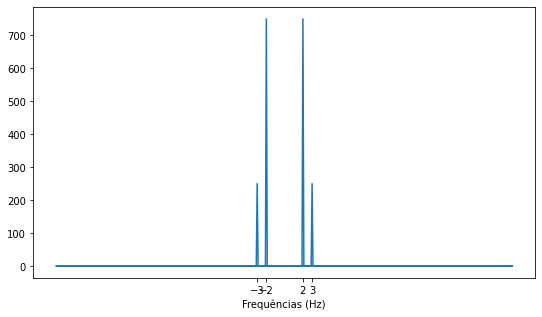
\includegraphics[width=1\textwidth]{./Imagens/Transformada de Fourier/TF2.png} 
	\caption{Picos de frequência}
	\label{fig:TF2}
\end{figure}

\subsubsection{Exemplo: Filtrando ruídos}
Vamos considerar um exemplo hipotético de um sinal dotado de ruídos e que originalmente veio da soma de dois sinais de frequências $50Hz$ e $120Hz$.

O sinal "limpo" sem ruídos é representado em cor vermelha, ao passo que o sinal com ruídos está na cor azul ciano.

\begin{minted}{python}
import numpy as np
import matplotlib.pyplot as plt

f, ax = plt.subplots(figsize=(12,5))

dt = 0.001

# vetor tempo de 1000 elementos, indo de 0 a 1
t = np.arange(0,1,dt)

# criando e somando senóides de frequência 50 e 120
f = np.sin((2*np.pi)*50*t) + np.sin((2*np.pi)*120*t)

# sinal resultante sem ruído
f_clean = f

# adicionando ruídos à soma
f = f + 2.5*np.random.randn(len(t))

# 1000
# print(len(f))

ax.plot(t,f, color='c', label = 'Sinal com ruídos')
ax.plot(t,f_clean, color='red', label = 'Sinal sem ruídos')
# setando um limite para o eixo x
plt.xlim(t[0],t[-1])
plt.legend()
plt.show()
\end{minted}

\begin{figure}[H]
	\centering
	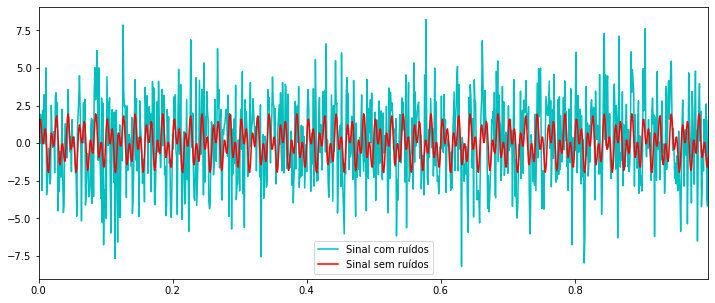
\includegraphics[width=1\textwidth]{./Imagens/Transformada de Fourier/TF3.png} 
	\caption{Sinal com e sem ruído}
	\label{fig:TF3}
\end{figure}

Vamos aplicar a \textbf{Transformada Rápida de Fourier} no sinal com ruído, plotar o resultado e trabalhar os dados de modo a eliminar a metade espelhada. Uma vez eliminada, obteremos um plot que nos exibirá as frequências correspondentes aos ruídos (frequências menores) e as frequências dos sinais componentes que deu origem ao sinal que queremos (picos de frequências). Aplicaremos, então, um \textbf{filtro} de modo a selecionar apenas as frequências maiores que $100Hz$ e eliminar os ruídos. Essas frequências filtradas serão submetidas, então, à \textbf{Transformada Discreta Inversa de Fourier} com o uso da função \textbf{ifft} para obtermos, por fim, o sinal limpo sem ruídos.

\begin{minted}{python}
# 1000
n = len(t)

# Transformada discreta do sinal com ruído
# O resultado é um array de números complexos
fhat = np.fft.fft(f,n)

# Multiplicando cada número complexo pelo seu conjugado
# PSD é um vetor de números reais
PSD = fhat * np.conj(fhat) / n

PSD = PSD.real

# print(PSD[:10])
# 1000
# print(len(PSD))

freq = (1/(dt*n)) * np.arange(n)
# [0. 1. 2. 3. 4. 5. 6. 7. 8. 9.]
# print(freq[:10])
# 1000
# print(len(freq))

L  = np.arange(1, np.floor(n/2), dtype = 'int')
# 500
# print(np.floor(n/2))
# [490 491 492 493 494 495 496 497 498 499]
# print(L[-10:])
# 499
# print(len(L))
\end{minted}

Continuação...

\begin{minted}{python}

fig, axs = plt.subplots(4,1, figsize=(15,10))

# ajustando a distância vertical entre os plots
fig.subplots_adjust(hspace=0.6)

# Sinal com ruído e sem ruído
plt.sca(axs[0])
plt.plot(t,f, color = 'c', label = 'Sinal obtido')
plt.plot(t,f_clean, color='red',  label = 'Sinal desejado')
plt.xlim(t[0], t[-1])
plt.legend()

plt.sca(axs[1])
axs[1].set_xticks([0.05,0.12])
axs[1].set_xlabel("Frequências (Hz)")
plt.plot(t,np.abs(fhat), color = 'blue', 
label = 'Transformada discreta espelhada') 
# plt.xlim(freq[L[0]], freq[L[-1]])
plt.legend()

axs[2].set_xticks([50,120])
axs[2].set_yticks([100])
axs[2].grid(True, axis = 'y', alpha = 1 , 
color = 'black', which='both')
axs[2].set_xlabel("Frequências (Hz)")

\end{minted}

Continuação...
\begin{minted}{python}

plt.sca(axs[2])
plt.plot(freq[L],PSD[L], color = 'blue', 
label = 'Transformada discreta') 
plt.xlim(freq[L[0]], freq[L[-1]])
plt.legend()

axs[2].fill_between(freq[L], 100, 400, 
where=np.abs(PSD[L]) > 0j, facecolor='green', alpha=0.5)

# indices: vetor de valores booleanos
# vamos filtrar os ruídos e eliminar 
# aqueles com valores menores que 100
indices = PSD > 100
PSDclean = PSD + indices
# print(PSD[:51])
# print(PSDclean[:51])
fhat = indices * fhat
# Transformada inversa dos valores filtrados 
ffilt = np.fft.ifft(fhat)
axs[3].grid(True, axis = 'x', alpha = 1 , 
color = 'black', which='both')
plt.sca(axs[3])
plt.plot(t, ffilt, color = 'red', 
label = 'Sinal filtrado')
plt.xlim(t[0], t[-1])
axs[3].set_xlabel("Tempo (s)")
plt.legend()
plt.show()
\end{minted}

\begin{figure}[H]
	\centering
	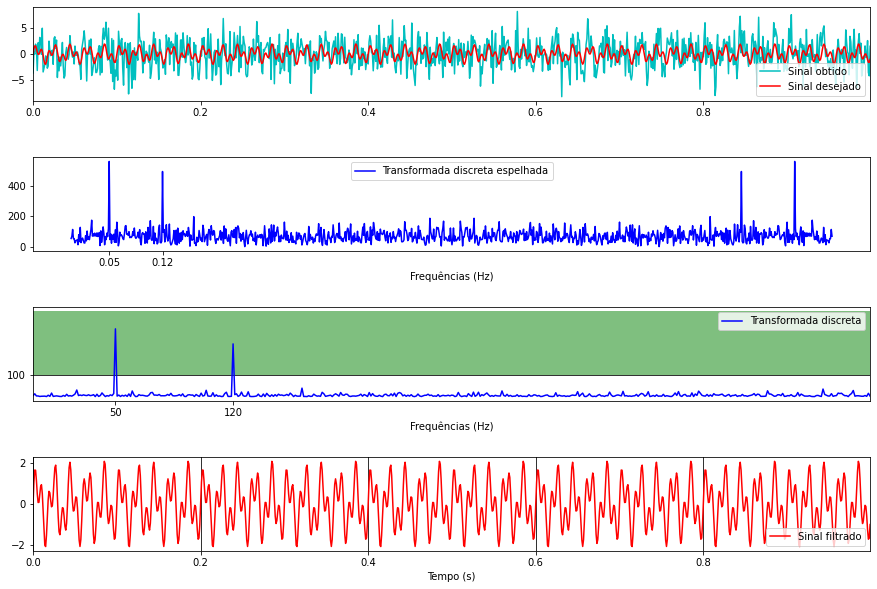
\includegraphics[width=1\textwidth]{./Imagens/Transformada de Fourier/TF4.png} 
	\caption{Sinal filtrado}
	\label{fig:TF4}
\end{figure}

Podemos ver que o sinal filtrado é exatamente igual ao sinal original sem os ruídos:

\begin{minted}{python}
import numpy as np
import matplotlib.pyplot as plt

f, (ax, ax2) = plt.subplots(2,1,figsize=(12,5))
dt = 0.0001
t = np.arange(0,0.1,dt)
f = np.sin((2*np.pi)*50*t) + np.sin((2*np.pi)*120*t)
n = len(t)
fhat = np.fft.fft(f,n)
PSD = fhat * np.conj(fhat) / n
PSD = PSD.real
freq = (1/(dt*n)) * np.arange(n)
indices = PSD > 100
PSDclean = PSD + indices
fhat = indices * fhat
ffilt = np.fft.ifft(fhat)
L  = np.arange(1, np.floor(n/2), dtype = 'int')
ax.plot(t,f, color='red', label = 'Sinal original')
ax.legend()
ax2.plot(t, ffilt, color = 'red', 
label = 'Sinal obtido a partir do sinal com ruído')
ax2.legend()
plt.show()
\end{minted}

\begin{figure}[H]
	\centering
	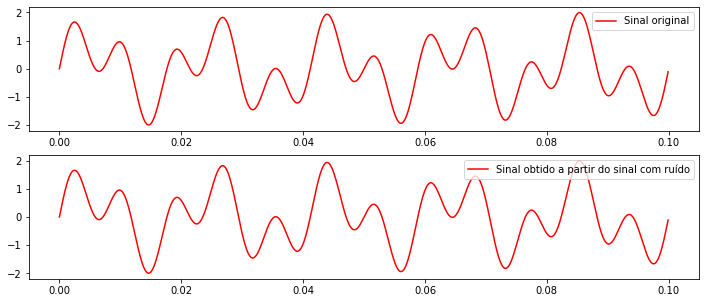
\includegraphics[width=1\textwidth]{./Imagens/Transformada de Fourier/TF5.png} 
	\caption{Comparação com o sinal original}
	\label{fig:TF5}
\end{figure}

\subsection{Aplicações da Transformada de Fourier}
\begin{itemize}
\item Processamento digital de sinais para a resolução de equações diferenciais parciais.
\item Em fones de ouvido com cancelamento de ruído. Ela converte o sinal original em componentes espectrais individuais e elimina os componentes indesejados.
\item Em processamento de imagens, sendo utilizado para decompor uma imagem em seus componentes seno e cosseno.
\item Na medicina, na técnica de Imagem por Ressonância Magnética.
\item Em óptica, no estudo da difração da luz quando ela passa por fendas estreitas. 
\item Na geologia e exploração de petróleo, na análise de dados sísmicos.
\end{itemize}